% TEMPLATE for Usenix papers, specifically to meet requirements of
%  USENIX '05
% originally a template for producing IEEE-format articles using LaTeX.
%   written by Matthew Ward, CS Department, Worcester Polytechnic Institute.
% adapted by David Beazley for his excellent SWIG paper in Proceedings,
%   Tcl 96
% turned into a smartass generic template by De Clarke, with thanks to
%   both the above pioneers
% use at your own risk.  Complaints to /dev/null.
% make it two column with no page numbering, default is 10 point

% Munged by Fred Douglis <douglis@research.att.com> 10/97 to separate
% the .sty file from the LaTeX source template, so that people can
% more easily include the .sty file into an existing document.  Also
% changed to more closely follow the style guidelines as represented
% by the Word sample file. 

% Note that since 2010, USENIX does not require endnotes. If you want
% foot of page notes, don't include the endnotes package in the 
% usepackage command, below.

\documentclass[letterpaper,twocolumn,10pt]{article}
\usepackage{usenix,epsfig,endnotes,graphicx,subcaption,url,breqn,enumitem}
\begin{document}
%don't want date printed
\date{}

%make title bold and 14 pt font (Latex default is non-bold, 16 pt)
\title{\Large \bf MochiDB : A Byzantine Fault Tolerant Datastore}
\author{
{\rm Tigran Tsaturyan}\\
Stanford University
\and
{\rm Saravanan Dhakshinamurthy}\\
Citrix Systems
}

\maketitle

% Use the following at camera-ready time to suppress page numbers.
% Comment it out when you first submit the paper for review.
\thispagestyle{empty}


\subsection*{Abstract}
In this paper we would like to present MochiDB - a consistent, high volume, distributed datastore which is Byzantine fault tolerant. MochiDB supports native transactions and uses BFT quorum protocol with random write seeds that requires only two round trips for writes and one for read which gives it low latency over WAN deployments. This paper puts focus on engineering solutions that minimize the cost of contention resolution, sharding, dynamic configuration changes, garbage collection and others. 

\section{Introduction}

Modern applications work across the globe serving million of users. Systems distributed over a shared network were fraught with limitations. The CAP theorem \cite{CAP_theorem} revealed that distributed systems can have at most two out of the following desirable properties - consistency, availability and partition-fault tolerance. Distributed systems were built focusing on a subset of the CAP properties. Some designers focused on write availability and partition fault tolerance \cite{Dynamo}. Some on consistency and partition fault tolerance \cite{RAFT}. Some on consistency and availability \cite{MYSQL_replication}. Moreover, different systems put different importance on performance, scalability, power usage, system reliability and many others. 

When designing MochiDB we were pursuing the use case of having consistent key-value datastore located within data centers around the globe supporting large volumes of data and transactions. We builtin Byzantine fault tolerance (BFT) support so that the system can remain consistent even if some nodes are malicious or have failed arbitrarily. Our concrete application was a infrastructure manager which centrally contains configurations for servers, VMs, docker images, site certificates, passwords, etc - i.e. everything that is read more often that is updated. Such information need to be consistent because small divergence can cause misconfigurations of the infrastructure and failures. We provide transaction support as very often multiple items are updated together. MochiDB does not provide data encryption by itself, although it is very possible to extend such service.

\section{System Overview}
MochiDB consists of clients and servers that contain the distributed database where data is stored. We represent data as a key-value store, where to some string 'K' is assigned some string value 'V'. We do not put any limit on key and value length, but our expectations are that keys are less than 80 characters long and data can be up to dozen Mb. MochiDB works only on string key and string values. Clients execute transactions across servers to access data for read and write. Each transaction consists of a list of operations. Each operation can be READ, WRITE or DELETE. Table \ref{table-operations} on page \pageref{table-operations} describes their meaning.

\begin{table}[]
\centering
\caption{MochiDB client operations}
\label{table-operations}
\resizebox{\columnwidth}{!}{%
\begin{tabular}{|l|l|l|l|}
\hline
\multicolumn{1}{|c|}{\bfseries Operation} & \multicolumn{1}{c|}{\bfseries Input arguments } & \multicolumn{1}{c|}{\bfseries Result} & \multicolumn{1}{c|}{\bfseries Meaning} \\ \hline
READ & Key & Current value & Read data mapped to key \\ \hline
WRITE & Key, New value & Old value & Write new data to key \\ \hline
DELETE &  Key & Old value & Delete data for key \\ \hline
\end{tabular}
}
\end{table}

A Transaction in MochiDB is guaranteed to be executed atomically. However, the transaction cannot be rolled back and the effects can be undone only via a separate transaction. MochiDB does not allow the same object (key) to appear twice within the same transaction. Aside from initiating a transaction, Clients communicate with servers relevant to the sharding scheme, acquire grants, commit results and perform reties whenever necessary. Clients nudge slow servers to resync objects that were found to be stale during a transaction.

Communication between participants (clients and servers) occurs via messages. MochiDB employs key authentication to guarantee that messages originated from the stated senders. The entire communication channel used for messages, data can be encrypted using TLS at the transport layer.

MochiDB is built to tolerate byzantine failures with some of the servers in the cluster experiencing stop failures, while others return arbitrary data, no data or malicious data intended to corrupt the distributed datastore. Such requirement intuitively means that more servers will be required to maintain consistency compared to non-BFT version. The relationship between number of servers and number of faulty servers (or faulty replicas) is described using the following equation:
$N = 3*f + 1$  where N is number of servers required (*without any sharding - see section later) and f is the presumed number of faulty servers.

Due to the nature of BFT protocol, we have to store relatively large metadata for any object in our datastore. For example, we store WriteCertificate which is the union of all write Grants given to that object. Such large metadata can be of significant overhead and require additional storage. Moreover, a very large datastore might not fit into a single MochiDB server. To solve those issues, we introduced sharding - the possibility to split data across different machines. We present sharding more in depth in the subsequent sections. Nonetheless in a nutshell, we shard by keys when apply known and fixed hash function that maps key universe into hash outcome universe. Our hash outcome is 32-bit signed integer, which can be viewed as a ring, starting with 0x0 and ending at 0xFFFFFFFF. That ring is split into equal size partitions by tokens. We assign each server some set of tokens. With that scheme, during write the client talks to subset of servers which relates to specified key. 

MochiDB supports dynamic configuration changes. User Client with special privileges can add and remove servers without shutting down the system. But during transition phase, read and write operations are put on hold.

\subsection{Design Assumptions}
When building MochiDB we took several assumptions which helped us to simplify the system and optimize relevant components. Since MochiDB is deployed over WAN in different parts of the world, communication between nodes is physically limited by underlying network. For example, ping time between Tokyo and Barcelona is around the magnitude of 300 ms and between Paris and Los-Angeles 150 ms \cite{PingLatencies}. Those times are multiple order of magnitude faster than CPU execution time. That means that optimizing for less number of message round-trips is better than optimizing for processing time. Hence, using public key cryptography as well as cryptographically secured hash functions do not dramatically bog down the system's throughput. 

\section{Architecture}

Our system consists of clients \( C = \{ C_{1},C_{2}, ..., C_{X} \} \). And servers \( S = \{ S_{1}, S_{2}, ..., S_{N} \} \). Clients are servers are identified by random ID which is unique for each client and server. Each of the clients can communicate with any of the servers. Servers store data inside internal DB (datastore) and reply to the clients by defined protocol. Sometimes servers can initiate communication and talk to other servers, for example to perform garbage collection or synchronize missing data.  Diagram \ref{fig:system_view} visualize our architecture. Similar architecture is described in \cite{HQ_replication}.

MochiDB is an asynchronous system "where nodes are connected by a network that may fail to deliver messages, delay them, duplicate them, corrupt them, or
deliver them out of order, and there are no known bounds on message delays or on the time to execute operations." \cite{HQ_replication}

\begin{figure}
\caption{MochiDB System Diagram}
\small
Each of the clients uses MochiSDK to execute Mochi protocol. Each of the servers contains of business logic (BL) which is responsible for running protocol and DB (datastore) which contains objects and metadata.
\centering
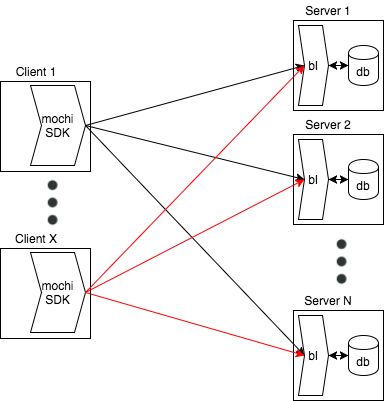
\includegraphics[width=0.35\textwidth]{System_View.png}
\label{fig:system_view}
\end{figure}

The server contains internal database (DB, datastore) which stores dynamic part of configuration, objects and metadata. DB is structured as keys mapped to StoreValueObjectContainers (SVOCs) and key represent object key. 
Internally SVOC stores value and metadata associated with object. For example, if MochiDB stores only two objects \(O_{1} = \{ "Washington":"Olympia" \} \) and \(O_{2} = \{ "California" : "Sacramento"\} \) which maps states to their capitals, then DB will contain two keys - {"Washington" and "California" }. Those keys will be mapped to some \( \{ SVOC_{1} \} and \{ SVOC_{2} \} \) respectively with values "Olympia" and "Sacramento" and metadata inside. The DB must support transactions and read-write object locking.

\subsubsection{SVOC and Object Metadata}
StoreValueObjectContainer contains the following data inside it:
\begin{itemize}[noitemsep, topsep=0pt,]
  \item \textit{value} - string value associated with that key. Can be null.
  \item  \textit{key} - string key for faster lookups
  \item  \textit{valueAvailable} - boolean property which indicates whether value is available. Non initialized or deleted keys will have valueAvailable set to false
  \item \textit{writeGrants} - list of hashmaps $\langle integer, writeGrant \rangle$. HashMap maps timestamp (TS) to write grant given on that timestamp. Such hashmap is one per epoch (see section \ref{Protocol_Writes}). DoubleLinked list keep hashmaps sorted by epoch.
  \item \textit{writeCertificate} - current write certificate for that object - i.e. signed collection of grants by different servers
\end{itemize}

\subsection{Model}

MochiDB model and design was largely influenced by HQ Replication \cite{HQ_replication}. Traditional agreement-based BFT protocols such as in \cite{Practical_BFT} requires too many message exchanges during operations between servers, but only one request and reply to the client. Such protocol performs well when servers are located close to each other and client is far. But in case of MochiDB, both servers and clients are located far from each other.

\begin{figure}
\centering
\begin{subfigure}[b]{0.45\textwidth}
   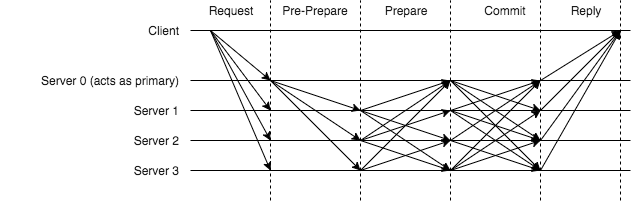
\includegraphics[width=1\linewidth]{Communication_agreement.png}
   \caption{Agreement based BFT}
   \label{fig:Ng1} 
\end{subfigure}

\begin{subfigure}[b]{0.45\textwidth}
   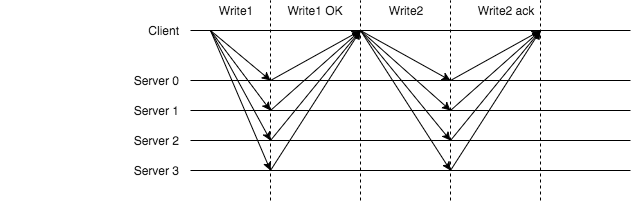
\includegraphics[width=1\linewidth]{Communication_quorum.png}
   \caption{Quorum based BFT}
   \label{fig:Ng2}
\end{subfigure}

\caption[Two numerical solutions]{(a) Agreement based BFT produces a lot of messages between the servers as well as require extra communication back to the client. Compared to (a) which requires less message and also less communications}
\end{figure}

Every time client perform read or write, it acts as a coordinator for transaction. Every read and write for an object has to be encapsulated as a transaction. In the best case scenario, we require only one round-trip for read transaction and two for write transaction. Read transactions do not modify state of the object. Write transaction consisting of only write operations does modify the state of the object. Write operations can be overriding value or deleting object. MochiDB puts constraint that we do not allow mix of read and write operations within the same transaction. That was done mostly for simplicity, but we believe that it is not hard to design such support in future. Client can perform multiple concurrent transactions, but they should not modify overlapping objects (reading while modifying is ok).

There is no guarantee of the outcome between concurrent transactions modifying the same objects. Let's assume that some transaction $T_{a}$ with one operation inside $O_{1} = \{write\ "valueA"\ to\ key\ "some\_key" \}$ and $T_{b}$ with one operation inside $O_{1} = \{write\ "valueB"\ to\ key\ "some\_key" \}$ are executed at the same time by multiple clients. After both succeed, it might be possible for value to be $"valueA"$ or $"valueB"$.

\subsection{Trust and Permissions}

During the message exchange it is critical that servers and clients identify the sender. Since servers and clients can lie in a byzantine environment, trusting incoming data is very naive approach. Moreover, it is possible for servers to re-transmit message from the client, effectively acting as a proxy. In such scenarios, we still might need to know the originator of the message to process it. To confirm that message was truly send by some party, MochiDB uses signatures.
Before the MochiDB cluster is setup, one must acquire a master certificate which will be used as trusted certificate authority. Such master certificate is fixed for the life of the cluster and must be carefully guarded. If such a certificate gets compromised then the cluster's security and data integrity is compromised as well. 
The Master certificate is used to sign certificates for every client and server in the MochiDB cluster. Whenever a client communicates with server, the server verifies that client's certificate is not blacklisted and the certificate is valid. Validation includes checking that certificate was truly signed by the master certificate. When client get response, it can validate the same for the server. MochiDB does not allow blacklisting server certificates, but it allows configuration change to remove faulty servers from the cluster.

MochiDB allows for the different permissions for different clients. Permission management is decentralized. When client is given certificate, it contains special property which defines permission level. We distinguish three level of permissions: READ (read objects), WRITE (read and ) and ADMIN (read, write objects and modify configuration). We expect that only one or few clients will be given ADMIN permission - the permission to add/remove nodes, blacklist certificates and modify sharding.

\section{Protocol Processing}
In the core of MochiDB lies quorum based BFT protocol. Most of the actions (read, write, epoch progressing, GC, etc.) are done in one or two phase approach. During phase one, some member (client or server) initiates action. It send it to all $3f+1$ nodes (Note: shading modifies that equation and is described separately. For the future descriptions assume that no sharding in present, unless specifically stated so). Then, the initiator waits for $2f+1$ (quorum size) matching responses for write and $f+1$ for reads. If server processing is required, then similar phase 2 starts: responses got during phase 1 are send back to the server along with some action. If something fails, initiator can suggest old servers to bring themselves up to speed and retry operation or message.
That mechanism is the foundation of every action. When we will be describing concrete actions (read, write, etc) you should expect to see some variety of that mechanism.

\subsection{Action}

Table \ref{table-actions} on page \pageref{table-actions} describes actions available in MochiDB.

\begin{table}[]
\centering
\caption{MochiDB actions}
\label{table-actions}
\resizebox{\columnwidth}{!}{%
\begin{tabular}{|l|l|l|}
\hline
\multicolumn{1}{|c|}{\bfseries Action} & \multicolumn{1}{c|}{\bfseries Initiator } & \multicolumn{1}{c|}{\bfseries Description } \\ \hline
Read & Client & Executes read transaction \\ \hline
Write & Client & Executes write transaction \\ \hline
NewEpoch & Client & Creates new epoch \\ \hline
GC & Server & Identifies objects to GC \\ \hline
ConfigModify & Client & Modifies configuration \\ \hline
UpToSpeed & Client/Server & Suggest replica to load latest data \\ \hline
\end{tabular}
}
\end{table}

\subsection{Reads}
Reads are initiated by client and their purpose is to read objects. Client creates read transaction and send readToServer message $\langle ReadToServer,\ transaction,\ nonce \rangle$ to all servers, where nonce is secure random number of uniquely identify request and avoid replay. Each of the servers reply back with readAns $\langle ReadAns,\ transactionResult,\ nonce \rangle$, where transactionResult contains list of OperationResult - one per each read operation. OperationResult has the format of ${result,\ currentCertificate, existed}$, where $result$ - string result of that operation, $existed$ boolean indicator whether such value existed and $currentCertificate$ is the current write certificate for that object.
Client waits for $f+1$ matching responses and if found, return $transactionResult$. If matches were not found, that indicates that some servers are not yet up to date. In that case, the client issues a message, asking server with older TS to bring it up to speed with other replicas. After a small wait time, the client retries the READ.
There is a risk that frequently updated keys will starve reads as there will be no quorum on the latest data. We assume that such possibility is low considering the use-case of our system but nonetheless we propose remedy for that - reading old stable data. Since the client has certificates for each conflicting object, it can downgrade object TS and perform read and that particular timestamp. That functionality put some implications on garbage collection and logic to bring servers up to speed and hence was left for the future work.

\subsection{Writes} \label{Protocol_Writes}
Write are initiated by the client and their purpose is to modify the state of objects. Writes are the challenging part of the protocol as concurrent modification of the same object needs to be coordinated. Some systems solve that issue by executing conflict resolution using agreement based BFT, which significantly increment number of messages \cite{HQ_replication}. In addition, while contention resolution is being processed, servers are frozen and do not serve requests \cite{HQ_replication}. Some other systems use dedicated primary and rotate it if selected one is faulty \cite{Practical_BFT}. Such system also suffers from number of messages and extra processing time for view change.
MochiDB uses randomness when performing write transaction thus significantly reducing the probability of collision and hence contention resolution. When collision happens, clients simply retry transaction with a new random seed number. That mechanism is described in details in section \ref{write_contension}. For now, let's see how write is processed without any contention.

Client initiate write transaction and send write1ToServer message $\langle Write1ToServer,\ transaction,\ transactionHash,\ subEpoch \rangle$ to all servers, where $transaction$ contains just the keys as values are unnecessary in the write1 phase, $transactionHash$ is the hash value calculated for the entire transaction including value (excluding value in case of delete) that will be stored in servers to authenticate the subsequent $Write2ToServer$ that will contain the complete key, value payload, $subEpoch$ is the random seed, a number within 0-1000 range alluded earlier in this paper. As the value payload will be sent later, $transactionHash$ is invaluable for servers to catch malicious clients who could flip the payload after aquiring a Write1Grant, by including it in the Write1Grant. Upon receiving write1 message, each server checks whether for each object there is already grant for timestamp $objectNextEpoch + subEpoch$, where $objectNextEpoch$ is the next timestamp epoch for that object and $subEpoch$ is the number it got from the client. MochiDB uses unsigned long format for timestamps. Each timestmap consist of epoch and numbering within epoch. We allocate 0-1000 for numbering within each epoch and the rest for epoch. For example, TS=4342 contains of epoch 4 (or equivalently, 4xxxx) and 342 as number within epoch. If timestamp is not granted to any other client, server creates write grant in form $\langle objectId, timestamp \rangle$. Grant is permission for that client to perform write operation on object X at specifies timestamp. Grants are not revocable - once granted, they can be executed at any point later on. Grants for all objects within transaction are unified under multiGrant and stored in the server so that the Server does not issue write1 grants to other clients and transactions overlapping our objects in the same timestamp. After stably storing multiGrant, server sends back write1ok message $\langle\ Write1OkFromServer,\ multiGrant,\ currentCertificates \rangle$ where $currentCertificates$ is hashmap mapping each object to its current certificate.

The client waits for $2f+1$ matching responses and construct $writeCertificate$ out of received multiGrants and send $\langle Write2ToServer,\ writeCertificate,\ transaction \rangle$ message to all servers. Servers processing Write2 message will verify whether the $writeCertificate$ contains $2f+1$ grants with consistent timestamps, calculate transaction Hash based on the complete $transaction$ and verify it with $transactionHash$ passed on Write1 phase, if all criteria are met, the Servers commit changes, save provided $writeCertificate$ as $currentCertificate$ for each object and delete the stably stored, corresponding write1Grant issued earlier in Write1 phase; the objects themselves might move to a new epoch if necesssary at the end of Write2 phase, more on that in the next section. If the Server finds a discrepancy in transactionHash or writeCertificate, the server rejects write2 operation and allows for the client to . In write2 phase, each server sends $Write2ack$ message with current state of object. The client can conculde the transaction is committed when it receives $2f+1$ matching $Write2ack$

If that grant with specified timestamp for object already exists, MochiDB checks whether clientId matches. If clientId matches, that is just retry of the same message and old result is returned. If clientId does not match that means that grant was given to somebody else and hence server sends back
$\langle\ Write1RefusedFromServer,\ currentCertificates,\\ availableSubEpochs\rangle$


\subsubsection{Write contention} \label{write_contension}
It is likely that two concurrent transactions will run at the same time and we will need a mechanism to resolve contention. MochiDB server does not freeze read, write requests to perform contention resolution. The random seed passed as $subEpoch$ minimizes the probability of contention and if contention with concurrent transaction had happened nonetheless, it will ask client to retry with a $Write1RefusedFromServer$ message. On a key that is frequently written, it is possible for clients to receive grants with timestamps that don't match, in such scenarios, the client waits for short time and retries $Write1ToServer$ till it receives $2f+1$ grants with the same future timestamp to proceed to the next phase.
Each exiting object contains $currentCertificate$ with timestamp inside it. That timestamp consists of epoch and numbering within the epoch - subEpoch. Object moves from one epoch to another when write2 message is received and write1 messages are assigned from nextEpoch. Intuitively, epoch change acts as a synchronization point between transactions - if two transactions run at the same time, objects they modify should be from the same epoch. If one transaction runs after another finished, object should belong to different epochs. Within each transaction different objects might be from different epochs, but subEpoch should be exactly the same. Diagram \ref{fig:epochs_view} visualize epoch timeline. 

\begin{figure*}
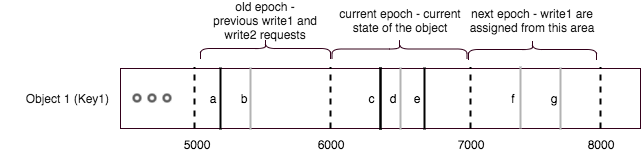
\includegraphics[width=0.8\textwidth]{Epochs.png}
\label{fig:epochs_view}
\caption{Object Epoch Timeline}
\small Object 1 has current epoch 6 $\left(6xxxx\right)$ because during that epoch the last write2 happened - points \textit{c} and \textit{e}. During epoch 6 write2 (point \textit{d}) was granted but never finished. Epoch 5 $\left(5xxxx\right)$ is old epoch with one finished write2 (point \textit{a}) and one non finished (point \textit{b}). New epoch is 7 $\left(7xxxx\right)$. Timestamps for write1 requests will be granted from that epoch. Currently two grants happened (points \textit{f} and \textit{g}), but no write2 was received yet.
\centering
\end{figure*}

When server executes write2 operations on old or current epoch, the following rule take affect:\\ If epoch of transaction T is less than current epoch - transaction will succeed, but no object will get modified. If epoch of T is the current epoch, but subEpoch is less that current committed subEpoch - Server does not modify the object, replies success along with most recent object value. If epoch of T is the current epoch, but subEpoch is large that current committed subEpoch - update current committed epoch, object write certificate, object value and return success. Such rules are enforced to allow for determinism if multiple commits happen within one epoch.

\subsubsection{Epoch exhaustion}
It is possible for too many concurrent writes exhaust 1000 range of numbers dedicated to it. If that happens, the clients can identify that and execute special protocol procedure which will start new epoch, without modifying current one.

\subsection{Garbage Collection}
MochiDB produces a lot of stored metadata (notably given Write1 grants) for every object in the datastore. To save disk space and prune expired Write1Grants, MochiDB uses Garbage Collection (GC). When performing GC, MochiDB treats objects independently. Each server runs a background thread that removes given Write1 Grants that were given 2 or more epochs before the current epoch. Recollect that we save Write1 Grant in server for every Object to avoid giving new Write1 Grant to a different transaction on the very same timestamp. As we have moved to newer epochs, the old write1 Grants are no longer needed as they had completed their purpose. Moreovoer, those expired Write1 Grants when cashed in future via Write2 will not lead to any object modifications. MochiDB server will recognize that the object timestamp acquired from its current certificate is greater than the grant timestamp in Write2 and therefore avoids modification of the object, as the object value had been superceded by clients with advanced timestamp grants. It responds back to late Write2 requests with Write2Ans that has the unmodified, latest object value.

\subsection{Resync}
Clients can detect slow mochiDB servers when they consistently issue write1 Grants that are from older epochs from the rest of the cluster. When alterted by a client with an $UptoSpeed$ operation, the slow mochiDB server acquires write locks on those objects so that all read, write operations pertaining to them stall and proceeds executes a special sync operation with an upto date mochiDB server identified by the client. This sync operation involves overwriting the identified set of objects' value, currentCertificate and given Wrie1 Grants to match those from the upto date server to complete the resync.

\subsection{Sharding}
MochiDB supports sharding natively. Each key is mapped to some hash by known and fixed hash function. All of available space is divided into equally sized partitions using Q tokens. Since hash space is known and the number of partitions fixed, it’s trivial and deterministic to calculate those tokens.
Each server is assigned multiple tokens by administrator depending on server performance, location to readers/writers, etc. That mapping is stored in the configuration of each server and also can be reliably retrieved by the client. When data is stored, it is stored on N nodes along the ring starting from the next token on the ring. The algorithm to determine nodes is the following:
\begin{enumerate}[noitemsep, topsep=0pt,]
  \item Apply hash to the key and get $H_{k}$
  \item Select the next token on the ring which follows or equals to $H_{k}$
  \item Circle the ring clockwise and select N nodes. Those will be the servers participated in transaction.
\end{enumerate}

Due to BFT requirements of the protocol, extra restrictions are added to the process above. N selected nodes = 3 f + 1, where f is number of faulty replicas. That has the following implications: If we want to double capacity (i.e. reduce by half number of partitions/shards on each server), in order to maintain the same f, we must double number of servers. Or if we reduced by half number of partitions on each server with the same amount of servers, we are also effectively reducing f.

Servers which are mapped to N selected tokens must be unique. That prevents the same faulty server participating multiple times in the transactions. That is fixable at the assignment time - when tokens are assigned to servers no 2 out of N sequential tokens are given to the same server.

\subsection{Configuration changes}
MochiDB allows configuration changes without reboot. Configuration is stored similar to other keys and all configuration keys starts with "CONFIG\_". We introduced “configurationstamp” (CS) which is a number, that increments every time configuration changes. During all operations (such as write1, write2, read, gc, etc.) CS is being passed alongside the message. The server denies message processing if its current CS differs from the received CS.

The following algorithm is executed on a client with admin privilege
\begin{enumerate}[noitemsep, topsep=0pt,]
\item Administrator allows all outstanding {UpToSpeed} actions to completion
\item Administrator sends config1 message to ALL servers. When servers receive config1, after validation they perform the following:
 \begin{enumerate}[noitemsep, topsep=0pt,]
    \item Checks whether there are concurrent config1 messages being processed at the moment. If there is one, the server will respond back with error. 
    \item Blocks server from accepting any new read, write messages.
    \item Send back config1ready
\end{enumerate}
\item The client waits for majority of config1ready messages, creates configChangeCertificate and proceed to phase 2.
\item During phase2, client send configChangeCertificate to each of the servers through config2 message. Upon receiving of message, each server will apply configuration, increment CS and reply with ack.
Configuration change assumed to be complete when client receives majority of acks
\end{enumerate}

\section{Implementation}
We built MochiDB using Java8, Netty as asynchronous network communication library, Protobufs as serialization library, Spring Boot for REST API and management UI. The functional, test and deployment code is over 48,000 lines and is publicly available in our open repository\cite{Repository}. We used in memory DB, but switching to some other DB (like MySQL) in future should be simple and uncomplicated. We have also published our in memory DB, mochiDB docker image \cite{DockerHub} for the public to test and deploy them in public cloud and enterprise data centers. Our implementation lacks PKI support - that work is left for the future, but our tests showed that adding TLS and signing messages should not have huge impact on the performance.  

\subsection{Evaluation}
During development we spun up virtual mochiDB server and client clusters within the JVM and built a test framework that tested the underlying sharding scheme, read, write, delete operations, concurrent transactions and a special stress test scenario. To evaluate the performance on a WAN setup, we devised 5 mochiDB clients concurrently executing transactions with a 5 node mochiDB Server cluster (sharded) running on AWS public cloud, us-west-1 zone. The average ping time between client and server clusters is about 13 ms. Each local client gets assigned 40 distinct keys and performs the following sequence of transactions : write key-value, then read each key and verify the content, followed by deletion of all keys. Table \ref{WAN-performance} on page \pageref{WAN-performance} describes read, write times measured. During this stress test, keys were assigned between clients without collisions. We noticed higher latencies for write and reads, when clients overlap keys used in their test execution.

\begin{table}[]
\centering
\caption{MochiDB WAN performance}
\label{WAN-performance}
\resizebox{\columnwidth}{!}{%
\begin{tabular}{|l|l|l|l|}
\hline
\multicolumn{1}{|c|}{\bfseries READ} & \multicolumn{1}{c|}{\bfseries Time } & \multicolumn{1}{c|}{\bfseries WRITE} & \multicolumn{1}{c|}{\bfseries Time} \\ \hline
50th percentile & 26.6 ms & 50th percentile & 56 ms \\ \hline
95th percentile & 31.1 ms & 95th percentile & 98 ms \\ \hline
99.9th percentile &  33.9 ms & 99.9th percentile & 145 ms \\ \hline
\end{tabular}
}
\end{table}

\section{Optimization}
We have identified that using leases will greatly improve write performance across the cluster and the use of hashes to reduce size of messages will improve the overall throughput. We can minimize metadata overhead, by only storing Grants pertaining to an object from majority of MochiDB servers instead of the all encompasing $writeCertificate$, that contains majority grants for all objects involved in the transaction.

\section{Conclusion}
In this paper we presented MochiDB - distributed, consistent, BFT key value store which is intended to work over high latency communication network. Our testing showed that MochiDB is a viable product that can work well for the situations with high read requests and moderate write requests. Our work is the first attempt to build a production ready BFT datastore for configuration management. In building MochiDB, we applied several enhancements to quorum based protocol including introduction of random write seeds and epochs to minimize contention resolution costs on the server.

{\footnotesize \bibliographystyle{acm}
\bibliography{mochiDB}}
\end{document}







